\chap{Постановка задачи}

	Целью данного исследования является разработка программного решения, подтверждающего принципиальную возможность и целесообразность построения и использования системы логического вывода в интеллектуальном управлении группой лифтов.

\section{Автоматическое доказательство теорем}
Одним из подходов к интеллектуализации систем управления является разработка алгоритмов обработки информации, основанных на моделировании процесса рассуждений. Наиболее формализованные подходы базируются на автоматическом построении логического вывода в некоторой системе формализованных знаний (логического описания предметной области). Программные системы для поиска логического вывода называют системами автоматического доказательства теорем (АДТ), поскольку утверждения, для которых существует логический вывод, являются теоремами (в заданном исчислении).

Для оценки систем АДТ используются следующие формальные критерии эффективности поиска логического вывода:

    \begin{itemize}
				\item[--] время решения задачи. Какое время затрачено системой АДТ для поиска логического вывода, либо установления факта невыводимости формулы;
				\item[--] количество шагов вывода. Количество шагов, из которых состоит найденный логический вывод (количество формул в цепочке);
				\item[--] расход памяти. Сколько памяти компьютера затрачено системой АДТ в процессе решения задачи;
				\item[--] ширина класса решаемых задач. Объединение класса новых задач решаемых системой и класса задач, для которых предложен новый способ решения.
    \end{itemize}
            
Очевидно, что повышение эффективности поиска логического вывода заключается в уменьшении численных характеристик критериев 1-3, и увеличении 4. 

\section{Позитивно-образованные формулы}
В качестве теоретического базиса разработанной системы АДТ выбрано исчисление позитивно-образованных формул (ПО-формул), созданное и исследованное под руководством академика С. Н. Васильева, канд. физ.-мат. наук А. К. Жерлова, на основе языка типово-кванторных формул, изначально использовавшегося для формализации свойств динамических систем и синтеза теорем в методе векторных функций Ляпунова.
Логическое исчисление состоит из трех компонент: язык, аксиомы и правила вывода. Далее представлены аксиомы и правила вывода. 
Исчисление ПО-формул имеет единственную аксиому и единственное правило вывода. Как и в методе резолюций, для доказательства формулы 𝐹 мы будем пытаться опровергнуть ее отрицание, поэтому аксиома исчисления ПО-формул — тождественно ложная ПО-формула вида ∀∅ (согласно принятым ранее сокращениям).
Для того, чтобы алгоритмы адекватно использовали возможности ПО-формализма необходимо выявить его совместимые полезные свойства, а также свойства, несовместимые с адаптируемыми алгоритмами. 
Существуют некоторые особенности формализма ПО-формул, которые необходимо разрешить для эффективной реализации системы АДТ. Анализ исчисления ПО-формул показал три основные проблемы (с указанием влияния на критерии эффективности, изложенные во введении):

    \begin{itemize}
				\item[--] поиск ответов на вопросы с неограниченными переменны- ми. Данная процедура требует выбора подставляемого терма для переменной вопроса из эрбранова универсума, который, в общем случае, т. е. при наличии функциональных символов, является счетным (бесконечным) множеством. Изначально неизвестно, какой именно терм необходимо выбрать, причем формально любая подстановка является корректной, хотя и не обязательно приводящей в итоге к опровержению формулы. В данном случае, решение проблемы направлено на повышение эффективности согласно критериям 1, 2;
				\item[--] язык ПО-формул в [4] характеризуется как «достаточно однородный, но в то же время хорошо структурированный», а соответствующее исчисление «хорошо усваивает эвристики», т. е. базовая стратегия исчисления достаточно легко настраивается под конкретную задачу. Стоит заметить, что представление ПО-формул использует большее разнообразие синтаксических структур, чем, например, представление дизъюнктов, которыми оперирует метод резолюций, в силу использования разнородных сущностей в структуре формулы: база, вопросы, консеквенты вопросов, два типа кванторов. То есть требуются применение специальных методов доступа к данным неоднородным частям ПО-формулы, а также разработка специальных структур данных представления ПО-формул. Решение этой проблемы направлено на повышение эффективности согласно критериям 1-3;
				\item[--] несмотря на то, что изначально представление формулы языка предикатов в языке ПО-формул более компактно чем КНФ, применение правила вывода в процессе построения логического вывода при наличии дизъюнктивного ветвления, в общем случае, приводит к бо́льшему усложнению структуры формулы, чем при применении правила резолюции. Таким образом, через некоторое количество шагов вывода размер ПО-формулы может оказаться в разы больше чем размер соответствующей КНФ. Другим фактором, присущим для всех методов и систем АДТ является неограниченная планка сложности решаемых задач. Некоторые формализации изначально являются весьма объемными. Отсюда вытекает потребность в обеспечении экономного использования оперативной памяти, а также обеспечение функционирования системы в режиме полного заполнения доступной памяти. Решение данной проблемы направлено на повышение эффективности согласно критерию 3;
				\item[--] для решения прикладных задач необходимо обеспечить настраиваемость системы АДТ для учета особенностей конкретной задачи.
    \end{itemize}

\section{Дерево состояний вывода}
Одним из основополагающих средств реализации поиска логического вывода в разработанной системе АДТ является дерево состояний вывода, которое строится, в основном, при помощи структур данных, базирующихся на чанках (рисунок \ref{dk6}).

        \begin{figure}[h]
				\centering
				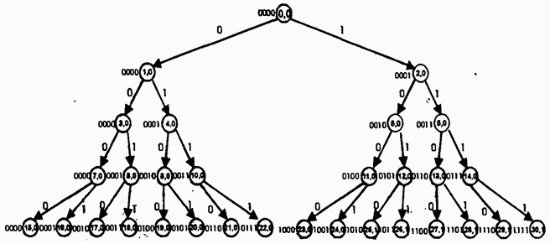
\includegraphics[width=150mm]{src/pictures/pic6.jpg}
				\caption{Дерево состояний}\label{dk6}
        \end{figure}
		% Рис. 6 - Дерево состояний
        
В структурах дерева состояний вывода, с одной стороны, хранится вся совокупность шагов вывода, по которой можно распознать какие действия были произведены на каком шаге. С другой стороны, дерево состояний вывода представляет текущую опровергаемую формулу. Основная задача дерева состояний вывода заключается в том, чтобы строго зафиксировать все события, произошедшие на каждом шаге логического вывода. Примером фиксируемого события является факт применения подстановки в базовой подформуле к некоторому вопросу. Такая фиксация событий позволяет:

    \begin{itemize}
				\item[--] использовать больше информации о выполненных действиях, тем самым анализировать процесс логический вывод, а значит эффективно (в смысле большего разнообразия вариантов управления) внедрять эвристики в базовую стратегию поиска логического вывода;
				\item[--] производить поиск логического вывода с возвратом (backtracking) в процессе построения логического вывода;
				\item[--] реализовать стратегию разделения данных (data sharing) для случая расщепления базовых подформул после ответа на вопрос с дизъюнктивным ветвлением;
				\item[--] производить эффективное (в смысле удобства реализации системы АДТ и производительности) управление оперативной памятью.
    \end{itemize}
    
\section{Системные предикаты и вычисляемые термы}
Разработка алгоритмов программной системы включает средства автоматизации анализа количественных и структурных характеристик процесса поиска логического вывода, а также средств управления логическим выводом. В результате реализации создана программная система АДТ и среда поддержки разработки систем АДТ, ориентированные как на практические задачи, так и на абстрактные задачи, традиционно считающиеся математическими.

В логических языках программирования, например, Прологе, введены так называемые системные предикаты (встроенные предикаты, built-in predicates), особенность которых заключается в том, что они в процессе построения ЛВ или выполняют некоторое побочное действие, например, вывод на экран, чтение файла и др., или их истинность вычисляется из значений параметров. Например, var(X) в Прологе определяет, является ли терм X переменной. Будем называть системным предикатом такой предикат, атомы которого входят в конъюнкты дерева ПО-формулы, но не участвуют непосредственно в ЛВ. Системные предикаты не имеют прямого отношения к формализации задачи, но они обладают одним из следующих свойств: они влияют на процесс ЛВ в результате реализации некоторых побочных действий; их истинностные значения вычисляются; они выводят некоторую системную информацию.

В системе реализованы следующие системные предикаты:

Next(L) — переход к вопросу, помеченному идентификатором L. Предикат помещается в конъюнкт корневой вершины консеквента вопроса. Если на данный вопрос будет произведен ответ, то следующим вопросом, для которого будет производится выбор ответа, будет вопрос (множество вопросов), помеченный идентификатором L. Таким образом, при помощи данного предиката задаются варианты порядка ответа на вопрос.

OffQuestion(L)/OnQuestion(L) — отключение/включение вопроса с идентификатором L. Отключенный вопрос объявляется неактивным, т. е. не принимает участие в логическом выводе, при этом в любой момент может быть заново включен.

RemQuestion(L) удаляет вопрос с идентификатором L. RemFact(L) и\\ RemPatternFact(L). Удаление факта помеченного идентификатором L, а также удаление  всех основных примеров L, если L –– терм.

OffFact(L)/OnFact(L) — отключение и включение факта с именем L. Поведение подобно включению и отключению вопросов.

Write(T) — печать терма T на стандартный вывод.

Save(L) — пометить состояние процесса поиска ЛВ в данной базовой подформуле идентификатором L.

Rollback(L) — откатить (backtrack) состояние вывода в базовой подформуле до состояния L с утерей более поздних по отношению к L маркировок.

Commit(L) — фиксировать состояние базы L как неоткатываемое, при этом фиксируются все состояния, помеченные ранее, чем L .
 
    
\section{Упрощения при реализации}
Поскольку в исследовании выявляется возможность и целесообразность построения и использования систем логического вывода, то при поиске решения допускаются все упрощения, которые неизбежны при построении моделей и при переходе к реальному приложению.

	Первым основным упрощением является дискретность времени с заданной величиной интервала между
		соседними моментами времени (тактами), содержащее начальный момент и бесконечно продолжимое вправо.
		Высота этажей считается одинаковой, и скорость движения лифта с одного этажа на другой полагаем
		равной одному такту. Длительность остановки кабин для входа-выхода пассажиров равняется одному такту.
		Так же не рассматриваются случаи переполнения кабин.

	Считается, что любой пассажир придерживается следующим правилам:
    
    \begin{itemize}
				\item[--] для вызова лифта он нажимает на этаже кнопку вызова и ждёт кабину, без ложных и ошибочных вызовов;
				\item[--] войдя в кабину, пассажир задаёт ей команду, для чего он нажимает кнопку нужного этажа, который вносится в маршрут данной кабины, без ложных и ошибочных команд.
    \end{itemize}

	Простейшим алгоритмом принятия решения является поиск ближайшей кабины к месту вызова.
		Однако, термин «ближайшая» требует уточнения и рассмотрения примера. 

	Допустим, есть система из k = 2 кабин, способных перемещаться по n = 5 этажам на рисунке \ref{dk7}.
		Пусть кабины находятся на 1-м и 2-м этажах, первая пуста и находится в покои,
		а второй предстоят остановки на 3-м и 4-м этажах. Поступает вызов с пятого этажа,
		и первая кабина получается ближайшей, так как её требуется 4 такта,
		а второй кабине требуется 5 тактов. Получается дистанция – это количество тактов,
		которое необходимо кабине, чтобы добраться до этажа, выполняя уже сформированный маршрут.
        
         \begin{figure}[h]
				\centering
				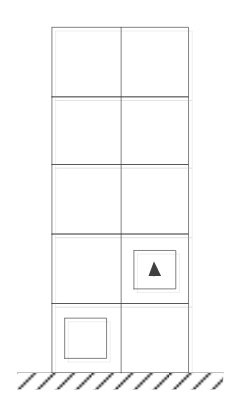
\includegraphics[width=70mm]{src/pictures/uproshenie.jpg}
				\caption{Интеллектуальное управление группой лифтов}\label{dk7}
    \end{figure}
		% Рис. 7 - Интеллектуальное управление группой лифтов

	Есть и другой подход, который основывается на исключении худших альтернатив на основе логического вывода.
		И если после сокращения допустимых альтернатив их останется несколько,
		то выбор может быть случайным или основываться на каких-либо критериях.
		В этом и предыдущих подходах одним из основных критериев является средняя длительность ожиданий.

\subsection{Логическая модель}
	Выстраивая логическую модель, получаем тройку (F, S, V), где F -- это позитивно образованная формула (ПОФ),
		описывающая состояние лифта и принципы, по которым функционирует лифт,
		S -- порядок ответов на запросы при логическом выводе, V -- внешние воздействие,
		в данном случае имитация пассажиропотока. Так же следует отметить, что одними из основных будут
		предикаты связанные со временем: T(t) -- момент времени t и N(t, t') -- следующий за t момент времени t'.

	Основными объектами в данной модели являются кабина Cab и человек Man.
		В момент времени t кабина имеет вид Cab(i, e, S, t), где i – идентификатор кабины, e – этаж,
		а S - маршрут кабины, список этажей. Человек имеет вид Man(e, d, τ, t), где e – этаж,
		d – целевой этаж, который добавляется в маршрут S в момент входа человека в кабину и d ≠ e,
		τ – длительность ожидания человеком кабины.
		Дистанцией же будет Dist(e, S, i, t, α), где α – это дистанция от кабины i
		на этаже е с маршрутом S, где произошёл вызов. И связь i кабины с вызовом с e этажа Conn(i, e).

	В каждый момент времени $t_0$ принятия решения формула F имеет вид\\

	$ \exists A(t_0) \begin{cases} \forall T(t)\exists T(t'), N(t, t'), \\ \Phi \\ \Psi \end{cases} $\\

	$A(t_0)$ -- коньюнкт, описывающий состояние системы в момент времени $t_0$. Если $A(t_0)$ содержит Man,
		то появление человека необходимо связать с вызовом определённой кабины.
		И группа формул \Phi порождает все варианты связи и имитирует движение кабин совместно с
		формулой времени $\forall T(t)\exists T(t'), N(t, t')$ для некоторого количества тактов.
		А за счёт формул \Psi происходит фильтрация некоторых вариантов.

	Оставшиеся варианты оцениваются оцениваются и выбирается один из самых наилучших.

	\subsection{Группа формул \Psi}

	$ \forall Man(e, d, τ, t), N(t, t')  \exists Dist(e, S_1, 1, t, \alpha_1), ..., \\
				Dist(e, S_k, k, t, \alpha_k)\begin{cases}\exists  Conn(1,e) \\ ... \\\exists  Conn(k, e), 
					\\\exists  Man(e, d, τ + 1, t') \end{cases} $\\

	-- формула вычисляющая дистанцию до каждой кабины при новом появлении человека

	$ \forall Cab(i, e, S, t), Conn(i, e'), N(t, t') \begin{cases}
			\forall e' < e \exists Cab(i, e - 1, S/e', t') \\
			\forall e < e' \exists Cab(i, e + 1, S/e', t')
	\end{cases} $


	$ \forall Cab(i, e, S, t), S = S(e', S_1), N(t, t') \begin{cases}
			\forall e = e' \exists Cab(i, e - 1, S_1, t') \\
			\forall e' < e \exists Cab(i, e - 1, S, t') \\
			\forall e < e' \exists Cab(i, e + 1, S, t')
	\end{cases} $


	$ \forall Cab(i, e, null, t), N(t, t')\exists Cab(i, e, null, t')$\\

	-- формулы реализующие движение, где $S / e$ является операцией вставки этажа в маршрут.

	\subsection{Группа формул \Phi}

	Формулы из группы \Phi реализуют дополнительные ограничения, которые следует учитывать при 
	построении логического вывода. В дальнейших работах они использоваться не будут. Но упомянуть о них
	крайне необходимо, так как они дают возможность данной модели быть более гибкой к различным ситуациям.
	А также их добавление в разрабатываемую систему не будет сложной задачей.

	Например, вот формула, которая запрещает откладывать связывание вызова лифта человеком белее, чем на 4 такта:

	$ \forall Man(e, d, 4, t)\exists False$

	Это правили необходимо, в том случае если в модели будет возможна отсрочка принятия решения на вызов лифта.

	Таким образом, определяется функция F. Её реализация будет выполнена на языке Prolog. Перевод из приведённых
	выше формул возможен по примеру из теоретической части.
